\documentclass[tikz,border=15pt]{standalone}
\usepackage{tikz}
\usetikzlibrary{arrows.meta, positioning, shapes.geometric}

\begin{document}
% Escala Real: 1 unidade no TikZ = 1 Metro.
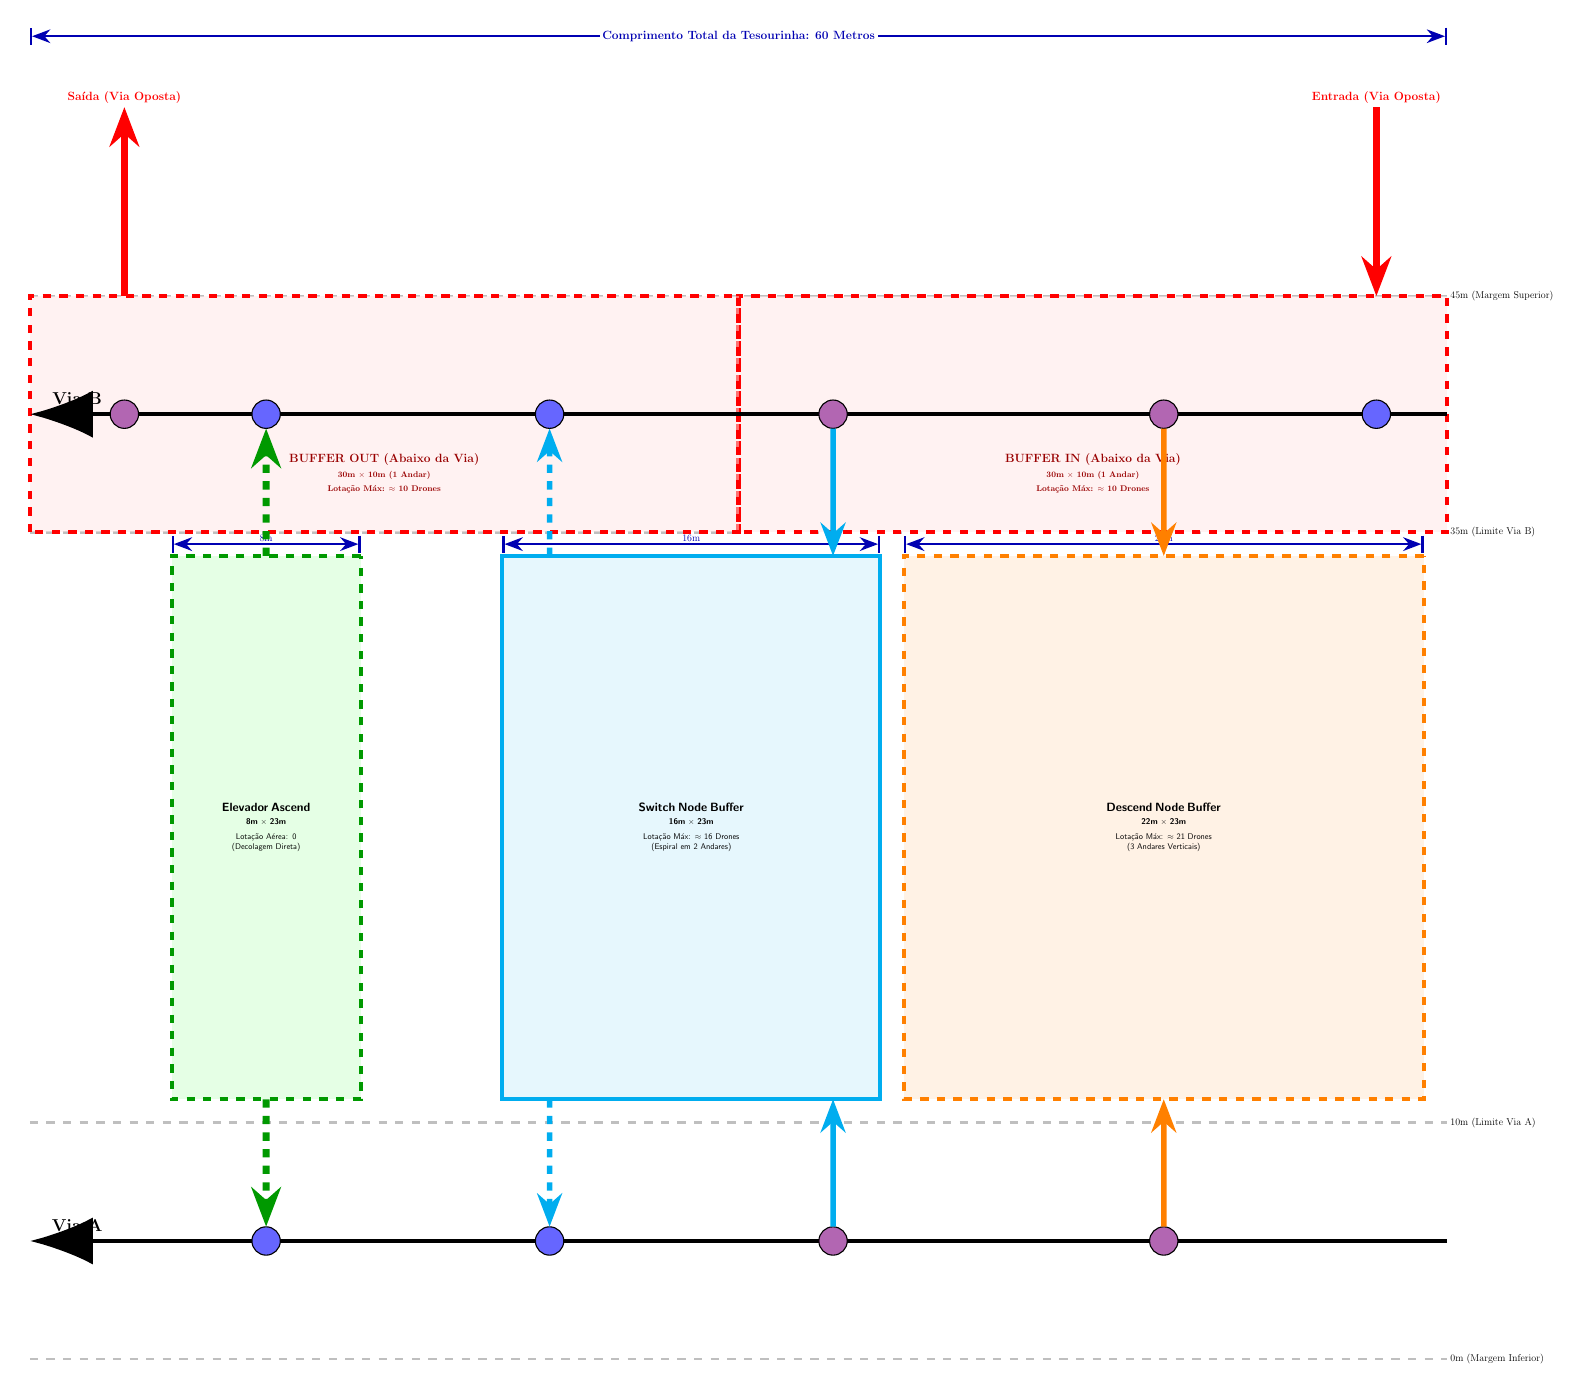
\begin{tikzpicture}[
    scale=0.3, transform shape,
    >=Stealth, 
    font=\sffamily,
    % Estilos das Linhas
    linha_principal/.style={draw, ultra thick, -{Latex[length=8mm, width=6mm]}},
    linha_cota/.style={|<->|, thick, blue!70!black},
    % Estilos dos Nós Táticos (Layer 2)
    no_purple/.style={circle, draw, fill=violet!60, minimum size=1.2cm, inner sep=0pt},
    no_blue/.style={circle, draw, fill=blue!60, minimum size=1.2cm, inner sep=0pt},
    % Estilos das Caixas de Buffer Central
    caixa_orange/.style={draw=orange, dashed, line width=1.5pt, fill=orange!10, align=center},
    caixa_cyan/.style={draw=cyan, line width=1.5pt, fill=cyan!10, align=center, font=\sffamily},
    caixa_green/.style={draw=green!60!black, dashed, line width=1.5pt, fill=green!10, align=center},
    % Estilo das Caixas Sobrepostas (Under-Layer para os Buffers IN/OUT)
    caixa_red_under/.style={draw=red, dashed, line width=1.5pt, fill=red!10, fill opacity=0.5, text opacity=1, align=center}
]

% =========================================================================
% 1. ESCALA GEOMÉTRICA GERAL (Corredor: 60m x 45m)
% =========================================================================
\draw[gray!50, dashed, line width=1pt] (0,0) -- (60,0) node[right, black, font=\large] {0m (Margem Inferior)};
\draw[gray!50, dashed, line width=1pt] (0,10) -- (60,10) node[right, black, font=\large] {10m (Limite Via A)};
\draw[gray!50, dashed, line width=1pt] (0,35) -- (60,35) node[right, black, font=\large] {35m (Limite Via B)};
\draw[gray!50, dashed, line width=1pt] (0,45) -- (60,45) node[right, black, font=\large] {45m (Margem Superior)};

% Cota Global do Comprimento
\draw[linha_cota] (0, 56) -- (60, 56) node[midway, fill=white, font=\Large\bfseries] {Comprimento Total da Tesourinha: 60 Metros};

% =========================================================================
% 2. BUFFERS IN / OUT (LAYER 1 - DESENHADOS NO FUNDO SOB A VIA B)
% Segregação Y=35 a 45 (Não colide fisicamente com as zonas centrais Y=11 a 34)
% =========================================================================
% Buffer IN (Metade Direita: X=30 a 60)
\draw[caixa_red_under] (30, 35) rectangle (60, 45);
\node[font=\Large\bfseries, text=red!60!black, align=center] (buf_in_text) at (45, 37.5) 
    {BUFFER IN (Abaixo da Via) \\ \normalsize \textbf{30m $\times$ 10m} (1 Andar) \\ \normalsize Lotação Máx: $\approx$ 10 Drones};

% Buffer OUT (Metade Esquerda: X=0 a 30)
\draw[caixa_red_under] (0, 35) rectangle (30, 45);
\node[font=\Large\bfseries, text=red!60!black, align=center] (buf_out_text) at (15, 37.5) 
    {BUFFER OUT (Abaixo da Via) \\ \normalsize \textbf{30m $\times$ 10m} (1 Andar) \\ \normalsize Lotação Máx: $\approx$ 10 Drones};

% Setas Externas (Interação com a Via Oposta / Fora da Tesourinha)
\draw[<-, red, line width=2.5pt] (57, 45) -- (57, 53) node[pos=1, above, font=\Large\bfseries] {Entrada (Via Oposta)};
\draw[->, red, line width=2.5pt] (4, 45) -- (4, 53) node[pos=1, above, font=\Large\bfseries] {Saída (Via Oposta)};

% =========================================================================
% 3. VIAS PRINCIPAIS A e B (LAYER 2 - FLUXO CONTÍNUO)
% =========================================================================
% Via B (Centro = 40)
\draw[linha_principal] (60, 40) -- (0, 40);
\node[above=8pt, font=\huge\bfseries] at (2, 40) {Via B}; 

% Via A (Centro = 5)
\draw[linha_principal] (60, 5) -- (0, 5);
\node[above=8pt, font=\huge\bfseries] at (2, 5) {Via A};

% =========================================================================
% 4. NÓS TÁTICOS (Deslocados geometricamente para otimizar os 60m)
% =========================================================================
% Nós da Via B (Y=40)
\node[no_blue]   (B_merge_in) at (57, 40) {}; % X=57: Merge IN
\node[no_purple] (B_div_desc) at (48, 40) {}; % X=48: Diverge Pouso
\node[no_purple] (B_div_sw)   at (34, 40) {}; % X=34: Diverge Switch
\node[no_blue]   (B_merge_sw) at (22, 40) {}; % X=22: Merge Switch
\node[no_blue]   (B_merge_el) at (10, 40) {}; % X=10: Merge Decolagem 
\node[no_purple] (B_div_out)  at (4,  40) {}; % X=4:  Diverge OUT

% Nós da Via A (Y=5)
\node[no_purple] (A_div_desc) at (48, 5)  {}; 
\node[no_purple] (A_div_sw)   at (34, 5)  {}; 
\node[no_blue]   (A_merge_sw) at (22, 5)  {}; 
\node[no_blue]   (A_merge_el) at (10, 5)  {}; 

% =========================================================================
% 5. ZONAS DE MANOBRA CENTRAL (Espaço livre Y=11 a Y=34 - Altura 23m)
% =========================================================================

% 5.1 DESCEND NODE (22m x 23m) - Posição X=37 a 59
\node[caixa_orange, minimum width=22cm, minimum height=23cm, text width=20cm] (descend) at (48, 22.5) 
    {\Large \textbf{Descend Node Buffer} \\[4pt] \normalsize \textbf{22m $\times$ 23m} \\[6pt] Lotação Máx: $\approx$ 21 Drones \\ (3 Andares Verticais)};
\draw[linha_cota] (37, 34.5) -- (59, 34.5) node[midway, above, font=\large] {22m};

% 5.2 SWITCH NODE (16m x 23m) - Posição X=20 a 36
\node[caixa_cyan, minimum width=16cm, minimum height=23cm, text width=14cm] (switch_nd) at (28, 22.5) 
    {\Large \textbf{Switch Node Buffer} \\[4pt] \normalsize \textbf{16m $\times$ 23m} \\[6pt] Lotação Máx: $\approx$ 16 Drones \\ (Espiral em 2 Andares)};
\draw[linha_cota] (20, 34.5) -- (36, 34.5) node[midway, above, font=\large] {16m};

% 5.3 LAYER 0 / DECOLAGEM DIRETA (8m x 23m) - Posição X=6 a 14
\node[caixa_green, minimum width=8cm, minimum height=23cm, text width=7.5cm] (layer0) at (10, 22.5) 
    {\Large \textbf{Elevador Ascend} \\[4pt] \normalsize \textbf{8m $\times$ 23m} \\[6pt] Lotação Aérea: 0 \\ (Decolagem Direta)};
\draw[linha_cota] (6, 34.5) -- (14, 34.5) node[midway, above, font=\large] {8m};

% =========================================================================
% 6. FLUXOS VERTICAIS E HORIZONTAIS
% =========================================================================

% Pouso (Descend)
\draw[->, orange, line width=2pt] (B_div_desc.south) -- (48, 34); 
\draw[->, orange, line width=2pt] (A_div_desc.north) -- (48, 11); 

% Troca Espiral (Switch)
\draw[->, cyan, line width=2pt] (B_div_sw.south) -- (34, 34);
\draw[->, cyan, line width=2pt] (A_div_sw.north) -- (34, 11);
\draw[->, cyan, line width=2pt, dashed] (22, 34) -- (B_merge_sw.south);
\draw[->, cyan, line width=2pt, dashed] (22, 11) -- (A_merge_sw.north);

% Decolagem Direta (Sobe da Layer 0 direto para o Merge na Layer 2)
\draw[->, green!60!black, line width=2.5pt, dashed] (10, 34) -- (B_merge_el.south);
\draw[->, green!60!black, line width=2.5pt, dashed] (10, 11) -- (A_merge_el.north);

\end{tikzpicture}
\end{document}